
\begin{figure}
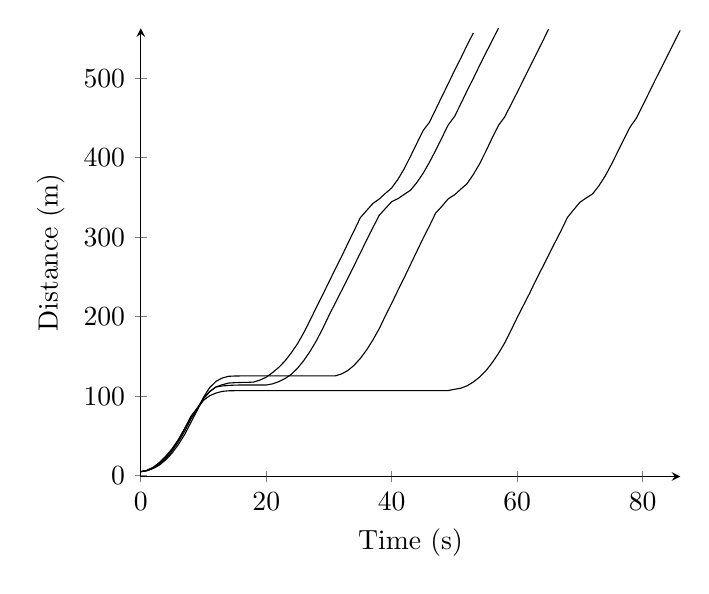
\begin{tikzpicture}
\begin{axis}[
legend style={anchor=west},
axis x line=bottom,
axis y line=left,
ymin=-1,
xlabel=Time (s),
ylabel=Distance (m),
]
\addplot[] coordinates {
(0, 5.1)
(1, 6.64222106969)
(2, 9.94255654825)
(3, 15.7302504873)
(4, 23.6353192297)
(5, 33.379443316)
(6, 45.1887858763)
(7, 59.4350025555)
(8, 74.7966906648)
(9, 85.2152263135)
(10, 97.2241338462)
(11, 105.750005963)
(12, 111.769393755)
(13, 114.49211613)
(14, 116.55111659)
(15, 117.043676059)
(16, 117.354416459)
(17, 117.383009974)
(18, 117.81049508)
(19, 120.292548524)
(20, 123.958485833)
(21, 129.701197686)
(22, 136.331608936)
(23, 144.482050155)
(24, 154.705375607)
(25, 166.274013191)
(26, 180.18181639)
(27, 195.724582889)
(28, 212.05201678)
(29, 227.642325169)
(30, 243.856610043)
(31, 259.846237641)
(32, 275.517362799)
(33, 292.093462785)
(34, 308.183157298)
(35, 324.64024541)
(36, 333.556809859)
(37, 342.41308433)
(38, 347.978104979)
(39, 355.137801269)
(40, 361.949760192)
(41, 372.916084516)
(42, 386.22616425)
(43, 401.884729026)
(44, 418.015419902)
(45, 434.00916194)
(46, 444.408025244)
(47, 460.626925681)
(48, 476.967886709)
(49, 492.936063015)
(50, 509.515279302)
(51, 524.997434187)
(52, 541.342761424)
(53, 556.75168424)
};
\addplot[] coordinates {
(0, 5.1)
(1, 6.36638545305)
(2, 9.30243288274)
(3, 13.5696476365)
(4, 20.1314546665)
(5, 28.6345690895)
(6, 39.2492282486)
(7, 51.976593022)
(8, 67.0245771441)
(9, 82.4604078064)
(10, 98.7163520405)
(11, 111.039071202)
(12, 118.773961062)
(13, 122.94910677)
(14, 125.04964648)
(15, 125.429905151)
(16, 125.519703096)
(17, 125.563282727)
(18, 125.573699004)
(19, 125.573699004)
(20, 125.573699004)
(21, 125.573699004)
(22, 125.573699004)
(23, 125.573699004)
(24, 125.573699004)
(25, 125.573699004)
(26, 125.573699004)
(27, 125.573699004)
(28, 125.573699004)
(29, 125.573699004)
(30, 125.573699004)
(31, 125.573699004)
(32, 128.007275839)
(33, 132.328488318)
(34, 138.853654755)
(35, 147.634846603)
(36, 158.223457604)
(37, 170.829468808)
(38, 184.828480358)
(39, 201.327349131)
(40, 217.005878856)
(41, 233.413011247)
(42, 249.249019426)
(43, 265.773341368)
(44, 282.193042867)
(45, 298.65954851)
(46, 314.02744358)
(47, 330.344659399)
(48, 338.858051333)
(49, 348.251658295)
(50, 353.190234554)
(51, 360.373157723)
(52, 367.224446396)
(53, 378.802082107)
(54, 392.215886112)
(55, 408.035253613)
(56, 424.541116503)
(57, 440.511305751)
(58, 451.192612492)
(59, 466.597250041)
(60, 482.174780299)
(61, 498.033788932)
(62, 514.010005337)
(63, 529.581405028)
(64, 545.524852281)
(65, 561.66929967)
};
\addplot[] coordinates {
(0, 5.1)
(1, 6.97163511669)
(2, 10.8694089052)
(3, 16.900412157)
(4, 24.7417281913)
(5, 34.0785144807)
(6, 45.4661569592)
(7, 59.1698752904)
(8, 74.1957297885)
(9, 84.3875896514)
(10, 94.8344252941)
(11, 100.700912106)
(12, 103.983952525)
(13, 106.135748401)
(14, 106.822095085)
(15, 106.968117599)
(16, 107.091838481)
(17, 107.112214046)
(18, 107.112214046)
(19, 107.112214046)
(20, 107.112214046)
(21, 107.112214046)
(22, 107.112214046)
(23, 107.112214046)
(24, 107.112214046)
(25, 107.112214046)
(26, 107.112214046)
(27, 107.112214046)
(28, 107.112214046)
(29, 107.112214046)
(30, 107.112214046)
(31, 107.112214046)
(32, 107.112214046)
(33, 107.112214046)
(34, 107.112214046)
(35, 107.112214046)
(36, 107.112214046)
(37, 107.112214046)
(38, 107.112214046)
(39, 107.112214046)
(40, 107.112214046)
(41, 107.112214046)
(42, 107.112214046)
(43, 107.112214046)
(44, 107.112214046)
(45, 107.112214046)
(46, 107.112214046)
(47, 107.112214046)
(48, 107.112214046)
(49, 107.112214046)
(50, 108.696177158)
(51, 110.050792627)
(52, 113.067467547)
(53, 117.849849469)
(54, 124.098211473)
(55, 131.935788912)
(56, 142.09842624)
(57, 153.700507823)
(58, 166.947656695)
(59, 182.620920027)
(60, 199.069400034)
(61, 214.431055725)
(62, 229.846550794)
(63, 246.295442149)
(64, 261.717822857)
(65, 277.387645225)
(66, 293.061378587)
(67, 308.411632281)
(68, 324.792633862)
(69, 334.591815677)
(70, 343.974781484)
(71, 349.29604795)
(72, 354.376098361)
(73, 364.430829375)
(74, 376.714779058)
(75, 391.27745209)
(76, 407.15177228)
(77, 423.21129805)
(78, 438.649458385)
(79, 449.78088942)
(80, 465.641566701)
(81, 481.655666947)
(82, 497.741303488)
(83, 513.404367087)
(84, 529.132781926)
(85, 545.035899547)
(86, 560.494393881)
};
\addplot[] coordinates {
(0, 5.1)
(1, 6.43195228846)
(2, 9.2931594038)
(3, 14.5785011656)
(4, 21.6156407485)
(5, 31.1473875431)
(6, 42.5569682803)
(7, 55.9834151961)
(8, 71.3790041248)
(9, 82.8418823935)
(10, 96.9242753689)
(11, 106.104233063)
(12, 111.585213671)
(13, 112.92004603)
(14, 113.605590807)
(15, 113.969860026)
(16, 114.108370079)
(17, 114.116752021)
(18, 114.116752021)
(19, 114.116752021)
(20, 114.116752021)
(21, 115.552020298)
(22, 118.355786037)
(23, 122.266965509)
(24, 127.623648608)
(25, 135.296234899)
(26, 145.071621791)
(27, 156.635245541)
(28, 169.900928896)
(29, 185.073676989)
(30, 201.663070318)
(31, 217.177160677)
(32, 232.746526147)
(33, 248.497642051)
(34, 264.230470112)
(35, 280.279303535)
(36, 296.398646086)
(37, 312.059565042)
(38, 327.476315526)
(39, 336.131200686)
(40, 344.705055833)
(41, 348.458489141)
(42, 353.863341166)
(43, 359.06835133)
(44, 368.677762075)
(45, 380.353809906)
(46, 394.031338469)
(47, 409.224755947)
(48, 425.114000724)
(49, 441.17092216)
(50, 451.654174038)
(51, 467.559095226)
(52, 484.000952333)
(53, 499.620920189)
(54, 515.917341001)
(55, 531.701974856)
(56, 547.082587066)
(57, 562.735248448)
};

\end{axis}
\end{tikzpicture}
\label{tik:0:82}
\caption{0 percent diving with GSC on route $82$}
\end{figure}
